\begin{frame}
	\begin{center}
		\begin{figure}
			\animategraphics[width=0.55\linewidth,loop,autoplay]{10}{images/gif01/frame-}{0}{6}
		\end{figure}
		\textcolor{blue}{\href{https://cloudsen12.github.io/}{https://cloudsen12.github.io/}}
	\end{center}
\end{frame}


\begin{frame}{CloudSEN12 - Team <3}
	\begin{center}
		\begin{figure}
			\centering
			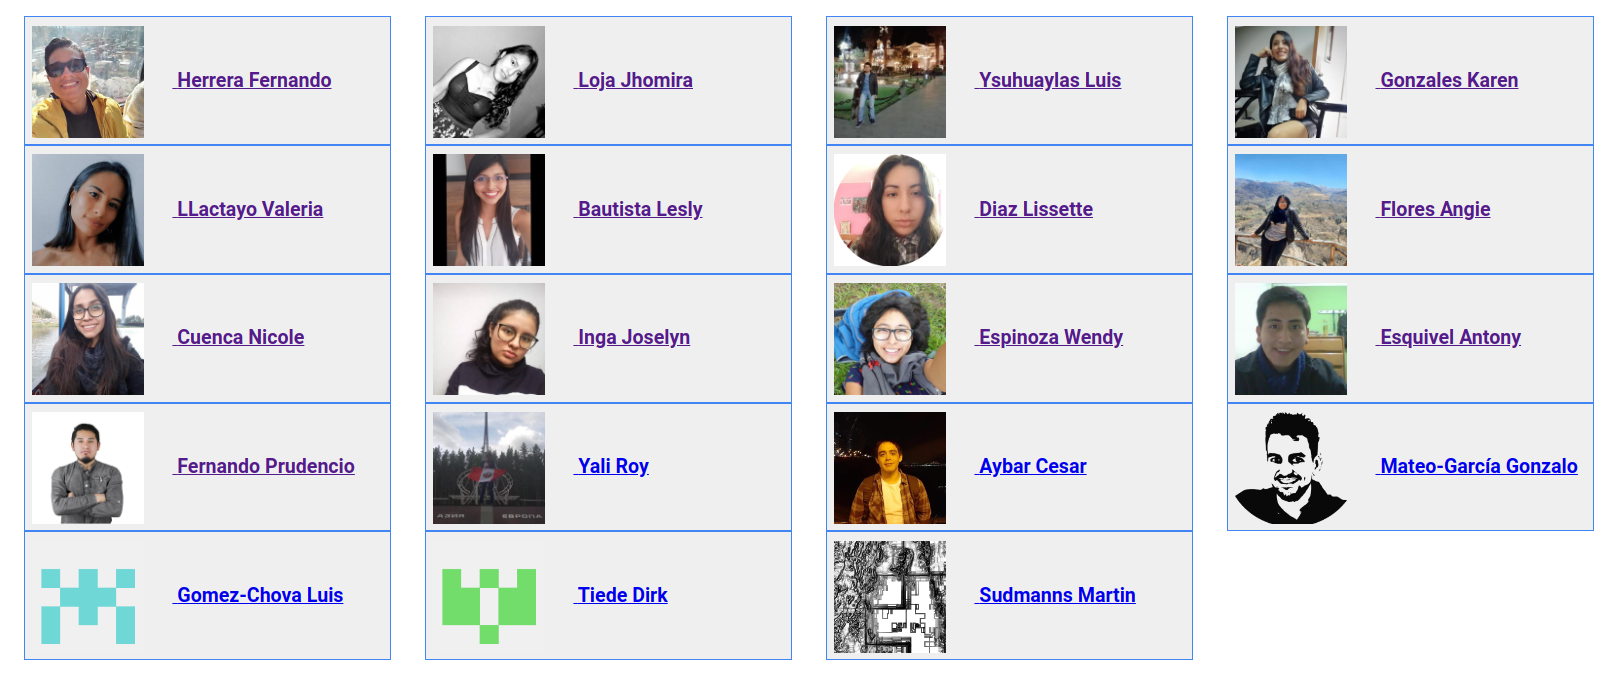
\includegraphics[width=1.0\linewidth]{images/dataset_team.png}
			{\caption*{CloudSEN12 team}}
			\label{fig:introfig01}
		\end{figure}
	\end{center}
\end{frame}


\begin{frame}{CloudSEN12 - Map}
	\begin{center}
		\begin{figure}
			\centering
			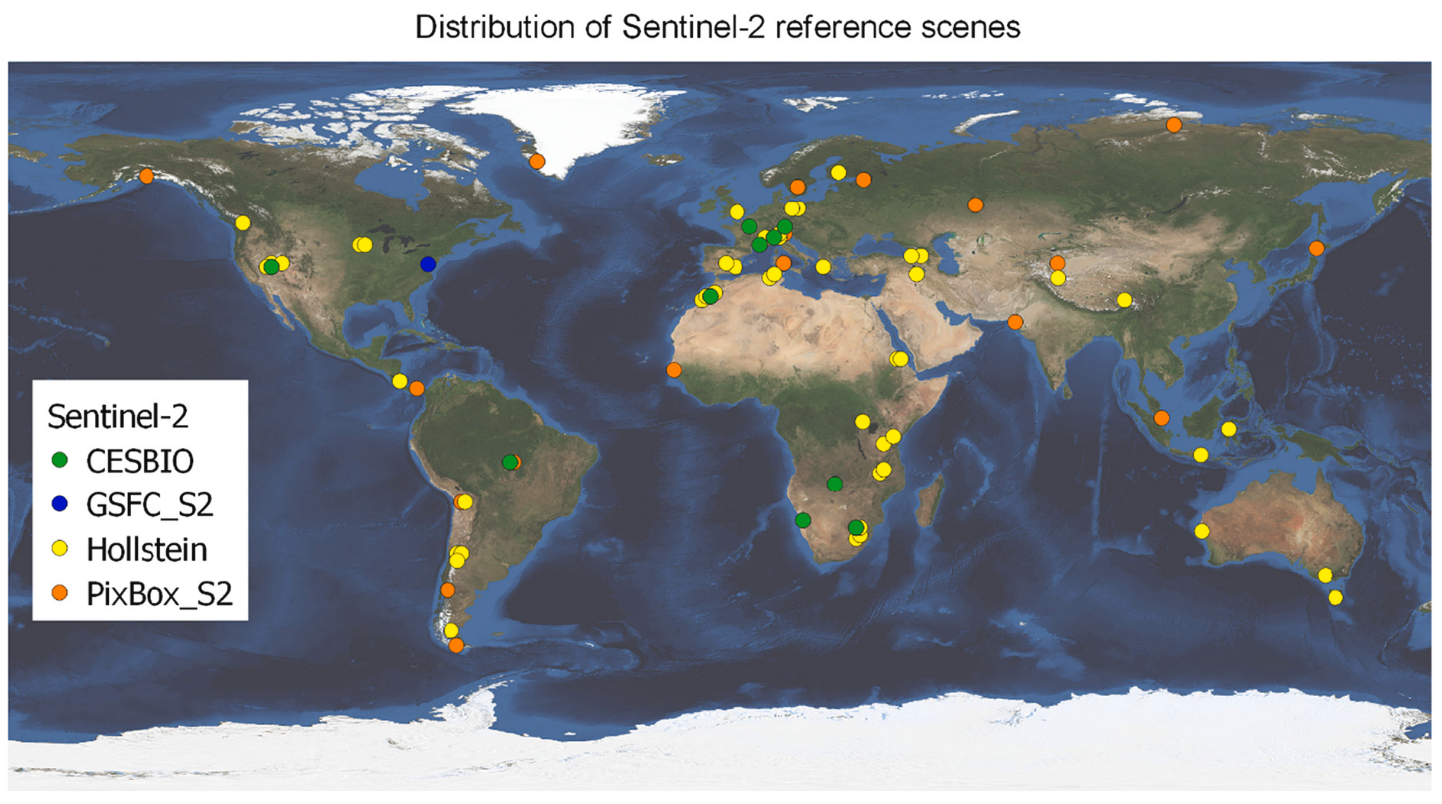
\includegraphics[width=0.85\linewidth]{images/intro_fig01.png}
			\caption[fig:introfig01]{Geographical distribution reference cloud detection datasets for Sentinel-2 (Skakun et al. 2022).}
			\label{fig:introfig01}
		\end{figure}
	\end{center}
\end{frame}

\begin{frame}{CloudSEN12 - Map}
	\begin{center}
		\begin{figure}
			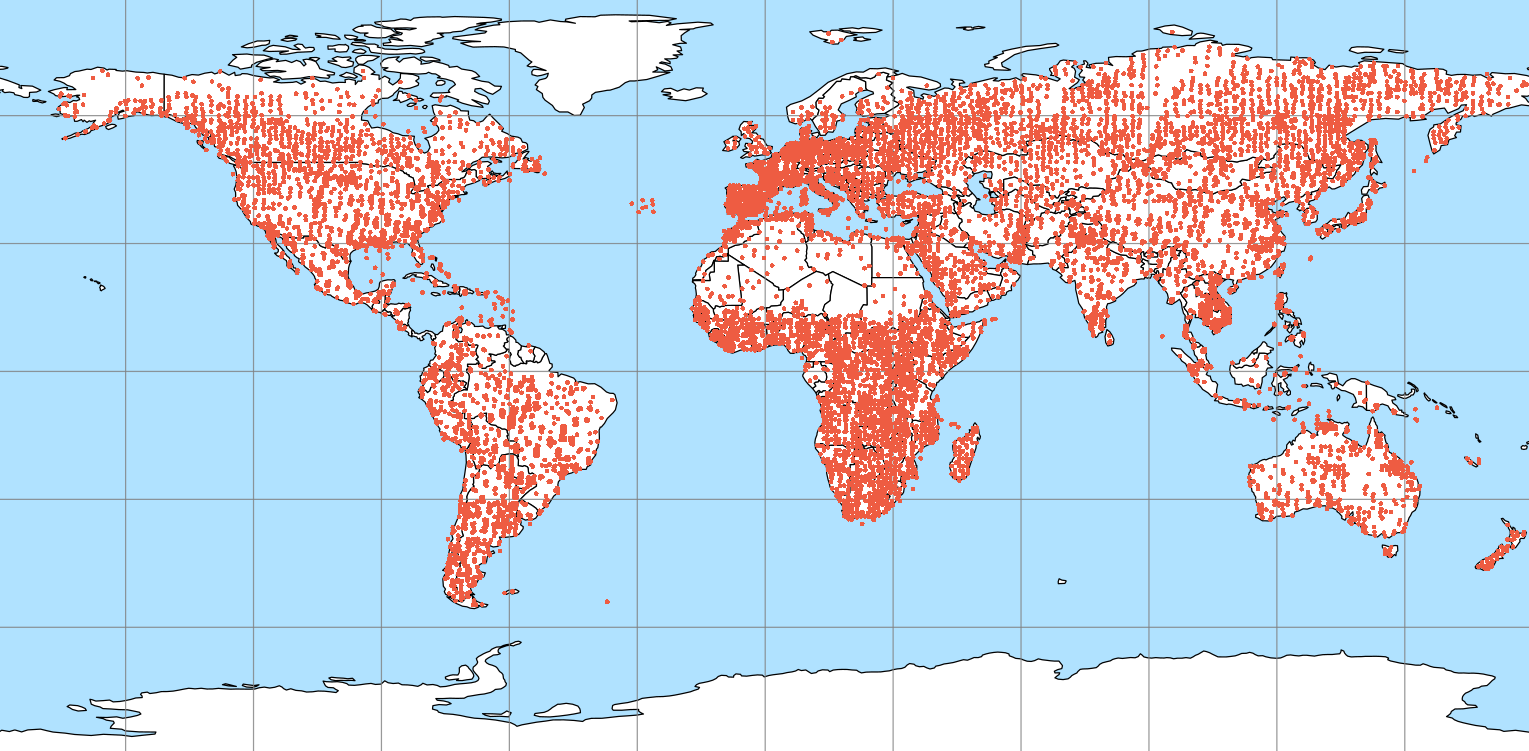
\includegraphics[width=0.85\linewidth]{images/intro_fig04.png}
			\caption[fig:introfig04]{CloudSEN12 spatial distribution}
		\end{figure}
	\end{center}
\end{frame}


\begin{frame}{CloudSEN12 - Data preparation}
	\begin{columns}
		\begin{column}{0.6\textwidth}
			\begin{figure}
				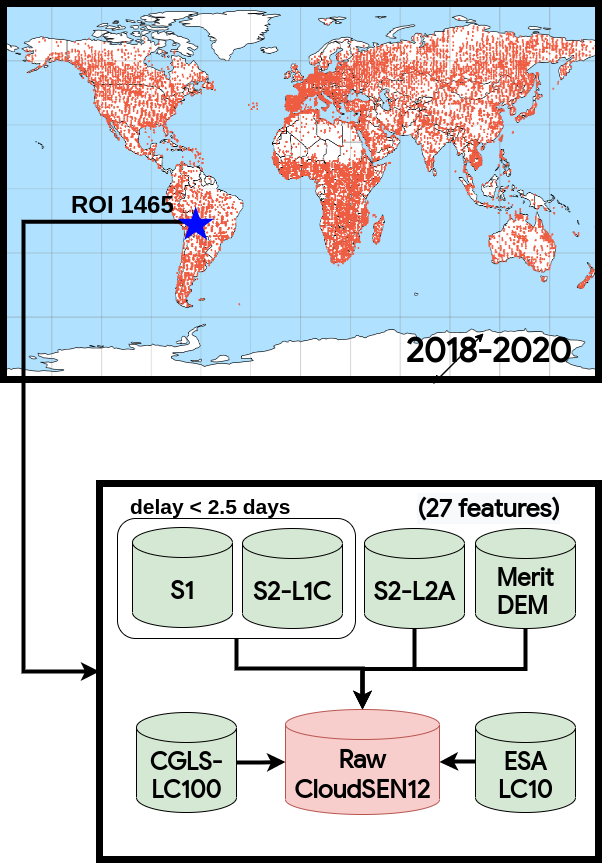
\includegraphics[width=0.6\textwidth]{images/methodology01.png}
				\label{fig:introfig02}
			\end{figure}
		\end{column}
		\begin{column}{0.4\textwidth}
			\begin{itemize}
				\item Merging of different spatio-temporal datasets to use as predictors.
				\item Semi-automatic selection of ROIs (5090x5090 m.)
			\end{itemize}
		\end{column}
	\end{columns}
\end{frame}




\begin{frame}{CloudSEN12 - Data Selection}
	\begin{columns}
		\begin{column}{0.7\textwidth}
			\begin{figure}
				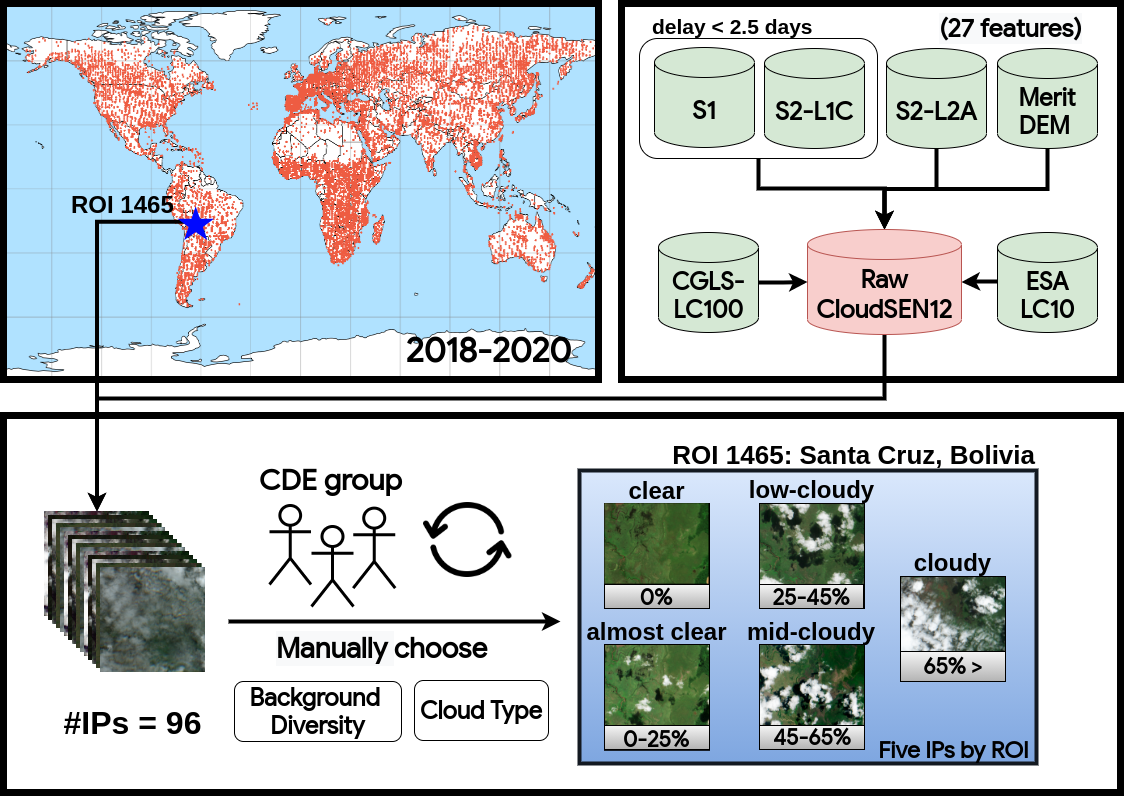
\includegraphics[width=1\textwidth]{images/methodology02.png}
				\label{fig:introfig02}
			\end{figure}
		\end{column}
		\begin{column}{0.3\textwidth}
			\begin{itemize}
				\item Each ROI have multiple IPs. We manually select five IPs considering the background, cloud type, and cloud coverage.
			\end{itemize}
		\end{column}
	\end{columns}
\end{frame}


\begin{frame}{CloudSEN12 - Labeling}
	\begin{columns}
		\begin{column}{0.7\textwidth}
			\begin{figure}
				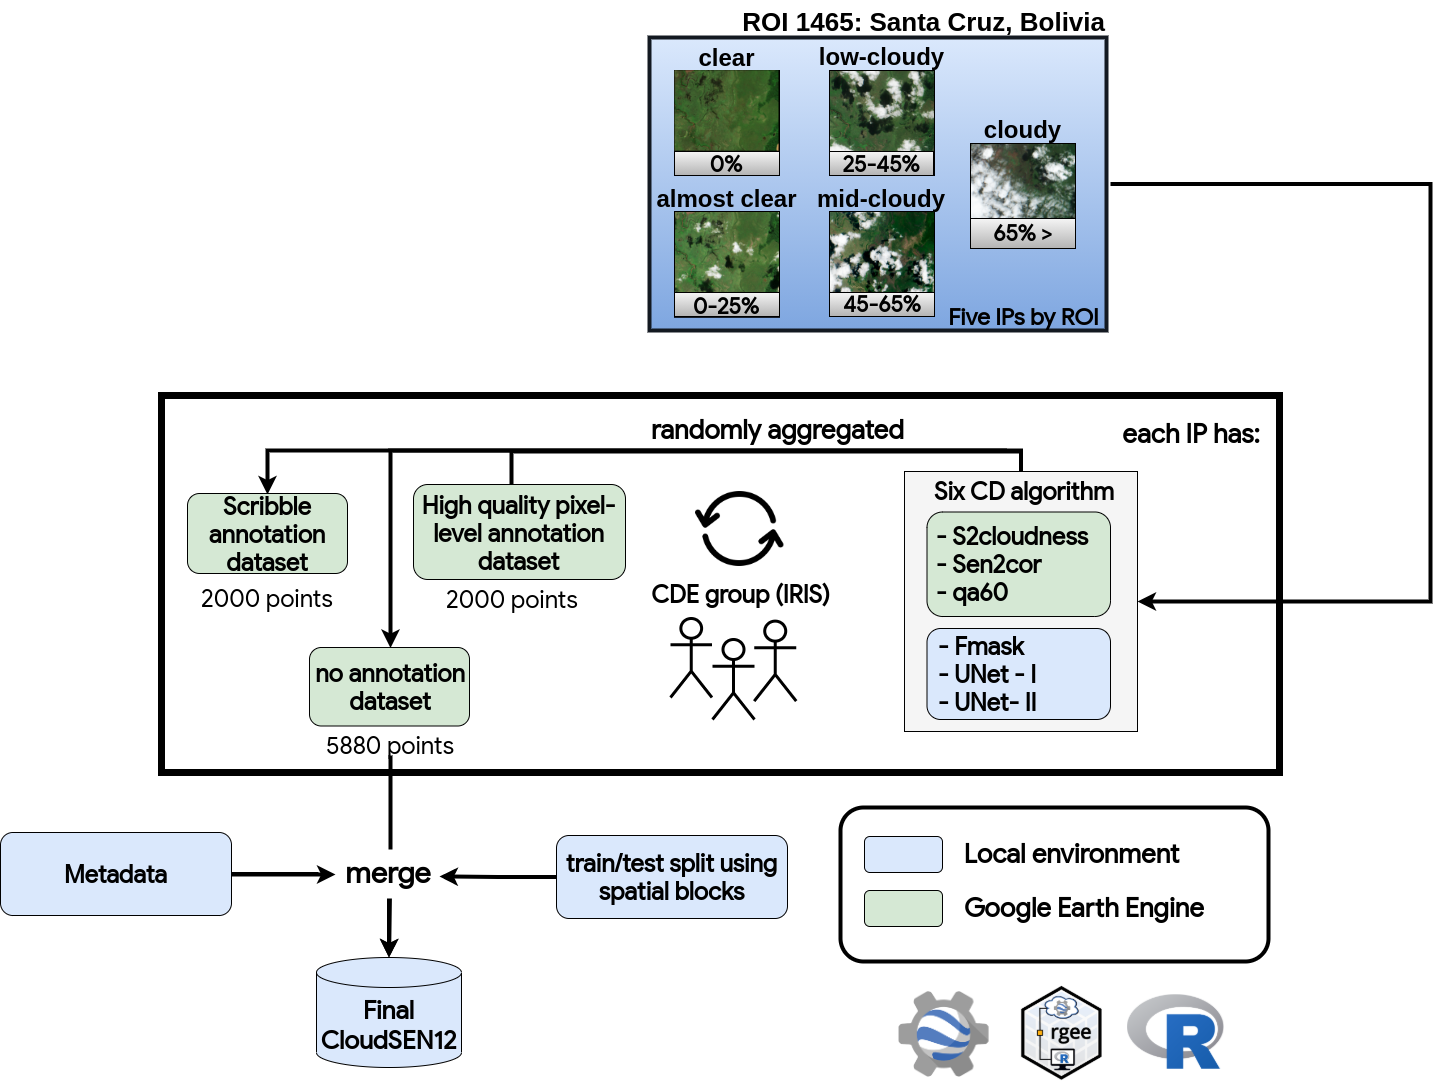
\includegraphics[width=1\textwidth]{images/methodology03.png}
				\label{fig:introfig02}
			\end{figure}
		\end{column}
		\begin{column}{0.3\textwidth}
			\begin{itemize}
				\item Add to each IP the results of 6 different CD algorithms. In addition, each ROI counts with manual labeling that can be of type: high-quality, scribble, or no annotation.
			\end{itemize}
		\end{column}
	\end{columns}
\end{frame}


\begin{frame}{CloudSEN12 - Labels}
\begin{figure}
	\centering
	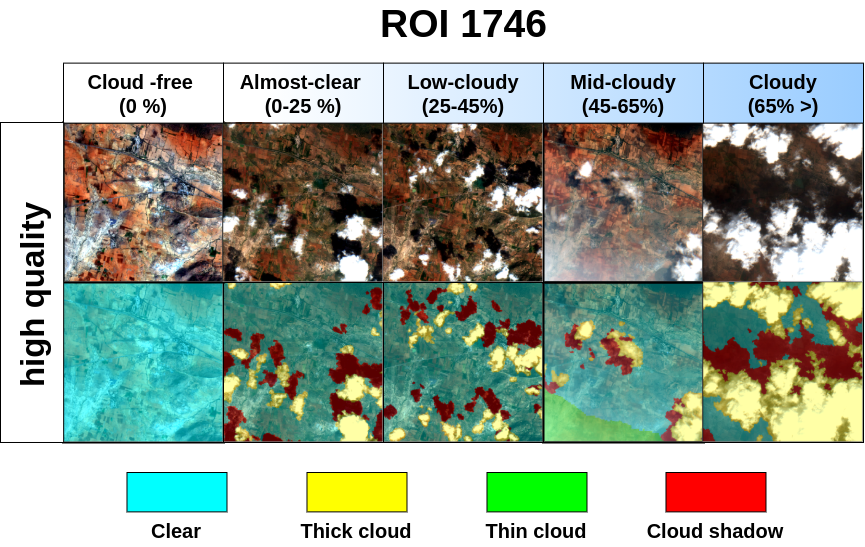
\includegraphics[width=0.7\linewidth]{images/labels01}
	\caption{}
	\label{fig:labels01}
\end{figure}
\end{frame}


\begin{frame}{CloudSEN12 - Labels}
	\begin{figure}
		\centering
		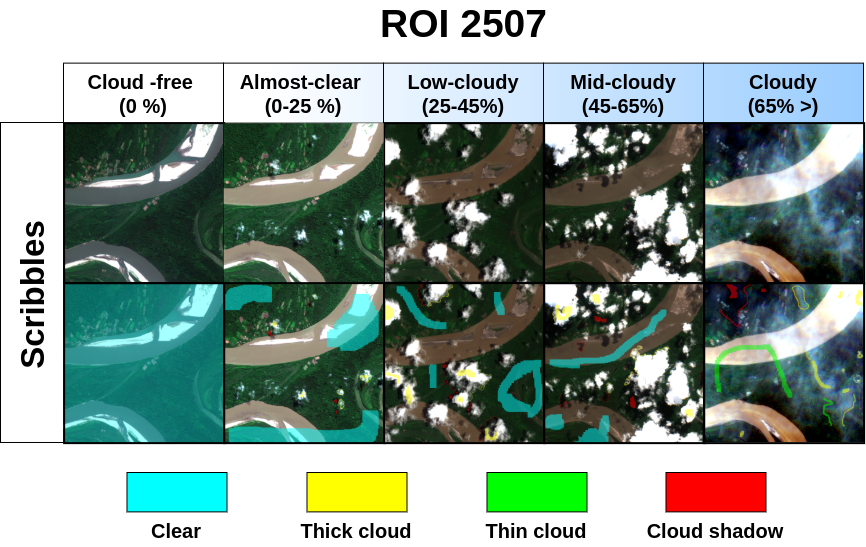
\includegraphics[width=0.7\linewidth]{images/labels02}
		\label{fig:labels01}
	\end{figure}
\end{frame}


\begin{frame}{CloudSEN12 - Labels}
	\begin{figure}
		\centering
		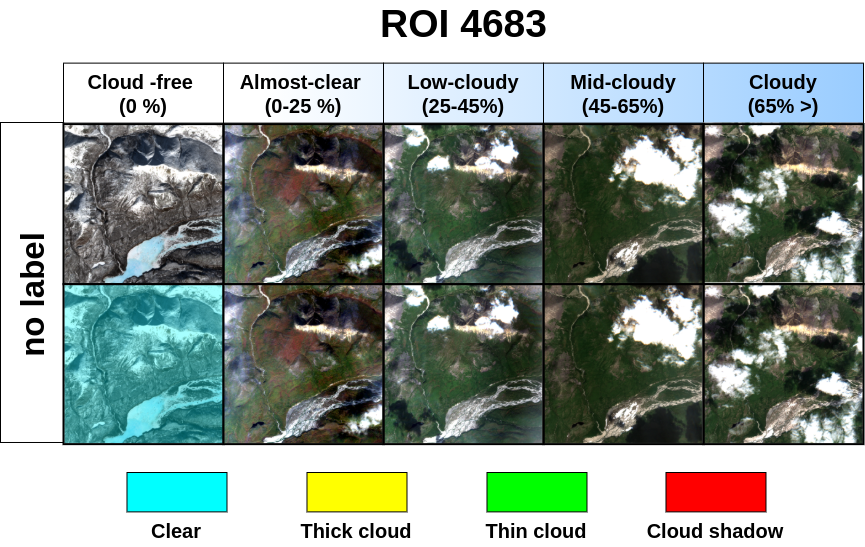
\includegraphics[width=0.7\linewidth]{images/labels03}
		\label{fig:labels01}
	\end{figure}
\end{frame}